\section{Experiments and Results}
\label{sec:coronary_experiments}

\subsection{Medical Data and Experimental Setup}
\label{subsec:coronary_setup_data}

The medical modality of the available original chest CTA series was a 128-slice Siemens SOMATOM Definition Flash CT.
The in-slice resolution was $0.4 \times 0.4 \text{mm}^2$ with slice thickness of $0.6 \text{mm}$.

Experiments were deployed with different parameters to segment the vasculature from CTA using our approach in this paper.
A desktop with Intel's 2.83GHz Core 2 Quad CPU and a RAM of four gigabytes served as the main workhorse.

To simplify the description, among the main branches of the coronary arteries, the 2D segmentation of the right coronary artery (RCA) in a typical slice is illustrated in this section.
The demonstrated approach can be straightforwardly applied to 3D segmentation of all the main branches of the vasculature.

\subsection{Preprocessing}

Since the focus of the work in this paper is on the coronary arteries, the ROI containing the whole heart needs to be extracted from the original chest CTA.
In our case, the coordination of the starting point and the spatial size of the ROI should be specified.
To keep the simplicity of the presentation, a typical slice was chosen to demonstrate this process (see Figure \ref{fig:coronary_ROI}).
\begin{figure}[!tb]
\centering
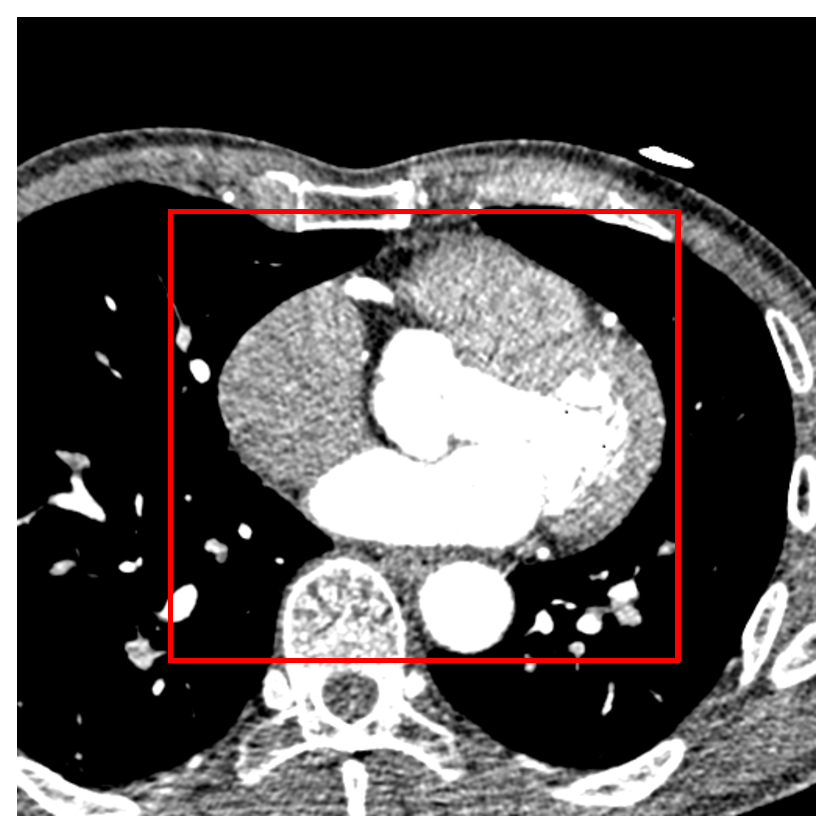
\includegraphics[width=2.8in]{Figures/coronary/ROI_Extraction}
\caption{ROI including heart region in original slice.}
\label{fig:coronary_ROI}
\end{figure}

After the ROI were successfully extracted, the aforementioned level-set curvature method with variable conductance \cite{Whitaker2001} was called to do the smoothing job.
The edge-preserving smoothing method attenuates the noises in the images without bringing in significant effects on the original boundaries of the vasculature.
As shown in Figure \ref{fig:coronary_smoothing}, the extracted image was nicely smoothed with the boundaries preserved.

To remove the irrelevant image details other than the coronary arteries per se, we adopted the general threshold filter with appropriately configured lower and upper thresholds (see Figure \ref{fig:coronary_threshold}). %
%This step can further facilitate the incoming processing jobs leading to the preservation of both time and space.
\begin{figure}[!tb]
\centering
\subfloat[]{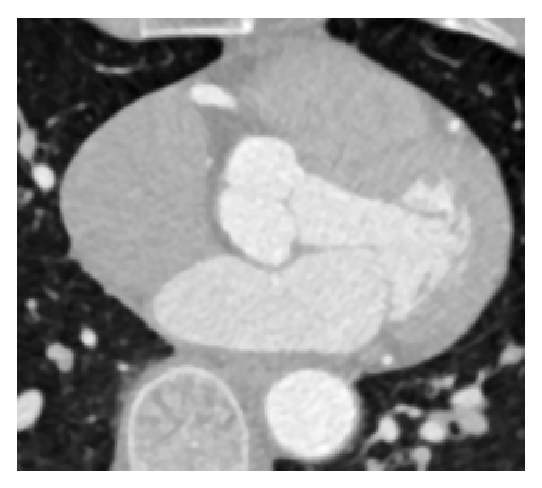
\includegraphics[height=2.5in]{Figures/coronary/smooth}%
\label{fig:coronary_smoothing}}
\hfil
\subfloat[]{
\includegraphics[height=2.5in]{Figures/coronary/threshold}%
\label{fig:coronary_threshold}}
\caption{Preprocessing results of original ROI: (a) smoothing with edge preservation ($\text{conductance} = 0.9$); (b) general thresholding ($\text{lower threshold} = 160$, $\text{upper threshold} = 600$).}%
\label{fig:coronary_preprocessing}
\end{figure}

\subsection{Image Features Computation}

In calculating the image features, the gradients at each pixel of the thresholded image were computed first.
Then the gradient map was mapped to the image feature map by applying the transfer function (\ref{eqn:coronary_sigmoid}).

The gradient magnitude module was utilized to perform the computation job in the first step.
The magnitude of the gradient was computed by performing convolution with the first order derivatives of a Gaussian kernel.
The only parameter of the kernel is its deviation $\sigma$ and we set it to 0.9.
As shown in Figure \ref{fig:coronary_gradient}, the edges of the vessels, and bones were thoroughly extracted.
After that, the intensity transformation was applied to shape the image feature map.
The choices of the parameters in (\ref{eqn:coronary_sigmoid}) relies on extreme values of the intensities in the gradient map.
To reverse the relationship between objects (in low intensities in the gradient map) and their edges (in high intensities in the gradient map), a negative $m$ was set whilst $n$ was set to be positive which is larger than $|m|$. %
The produced the image feature well met the expectations: lower on the edges and higher elsewhere (see Figure \ref{fig:coronary_sigmoid}).
This provided the fronts driven by (\ref{eqn:coronary_application}) with the guidance such that the fronts evolve faster in the area with uniformly high intensities, while much slower on the edges. %
\begin{figure}[!tb]
\centering
\subfloat[]{
\includegraphics[height=2.5in]{Figures/coronary/gradient}%
\label{fig:coronary_gradient}}
\hfil
\subfloat[]{
\includegraphics[height=2.5in]{Figures/coronary/sigmoid}%
\label{fig:coronary_sigmoid}}
\caption{Image features of the original CTA images: (a) gradient map by recursively using Gaussian kernel ($\sigma = 0.9$); (b) nonlinear intensity mapping by using an S-shaped transfer function ($m = -80$, $n = 120$), the minus sign of $m$ indicates the inverse mapping of the input intensities.}%
\label{fig:coronary_image_features}
\end{figure}


\subsection{Interface Propagation}

The initial level set contour was generated by evolving the contour from the user-provided seeding points.
The drive behind this evolution is provided by the fast marching algorithm.
The classic algorithm acquires one seeding point to start with.
During the computation, the contour evolves ``outwards" in order to detect the boundaries of the targeting objects.
As mentioned in Section \ref{subsec:coronary_setup_data}, RCA in this slice is the only targeting objects in this section.
In the case of 3D segmentation of the vasculature, multiple seeding points should be picked as input and all of them be located in the areas corresponding to the vasculature.
As shown in Figure \ref{fig:coronary_Fast_Marching}, the initial level set around the RCA in this slice is well generated for further processing.

The CURVES system started the computation once all the previous work completed.
The drive of the evolution is provided by (\ref{eqn:coronary_application}).
The image features supplied as the guidance map for the evolution whilst the initial level set generated by the fast marching method served as the initial state.
The fronts propagation stops only until the contour meets the edges of the spatial curve-shaped vasculature (see Figure \ref{fig:CURVES}).
After the evolution finished, the binary threshold filter was called to converse the intensities of the targets (RCA in the selected slice) and background.
The thresholded slice is illustrated in Figure \ref{fig:coronary_final}, the area corresponding to the RCA branch is in high intensities with black background.
\begin{figure}[!tb]
\centering
\subfloat[]{
\setlength{\fboxrule}{1pt}
\setlength{\fboxsep}{0cm}
\fbox{
\includegraphics[height=2.5in]{Figures/coronary/fastmarching}}%
\label{fig:coronary_Fast_Marching}}
\hfil
\subfloat[]{
\setlength{\fboxrule}{1pt}
\setlength{\fboxsep}{0cm}
\fbox{
\includegraphics[height=2.5in]{Figures/coronary/curves}}%
\label{fig:coronary_CURVES}}
\hfil
\subfloat[]{
\setlength{\fboxrule}{1pt}
\setlength{\fboxsep}{0cm}
\fbox{
\includegraphics[height=2.5in]{Figures/coronary/final}}%
\label{fig:coronary_final}}
\caption{Fronts propagation: (a) initial contour generated via fast marching algorithm; (b) contour evolution by using CURVES; (c) binary thresholded final contour.}%
\label{fig:Evolution}
\end{figure}

\subsection{Visualization of Segmented Data}

The computing surface, representing the inner wall of the coronary arteries tree structures, corresponds to the iso-surface extracted by using the marching cubes method \cite{Lorensen1987MC}.
The iso-surface information is based on the previous segmentation results generated by CURVES evolution.
As shown in Figure \ref{fig:coronary_CURVES_model}, the surfaces are well extracted and organized into the expected visualization model of the main branches of the coronary arteries tree.
To provide the model with an intuitive visualization effect, part of the root of the aorta is also extracted and visualized.
\begin{figure}[tb]
\centering
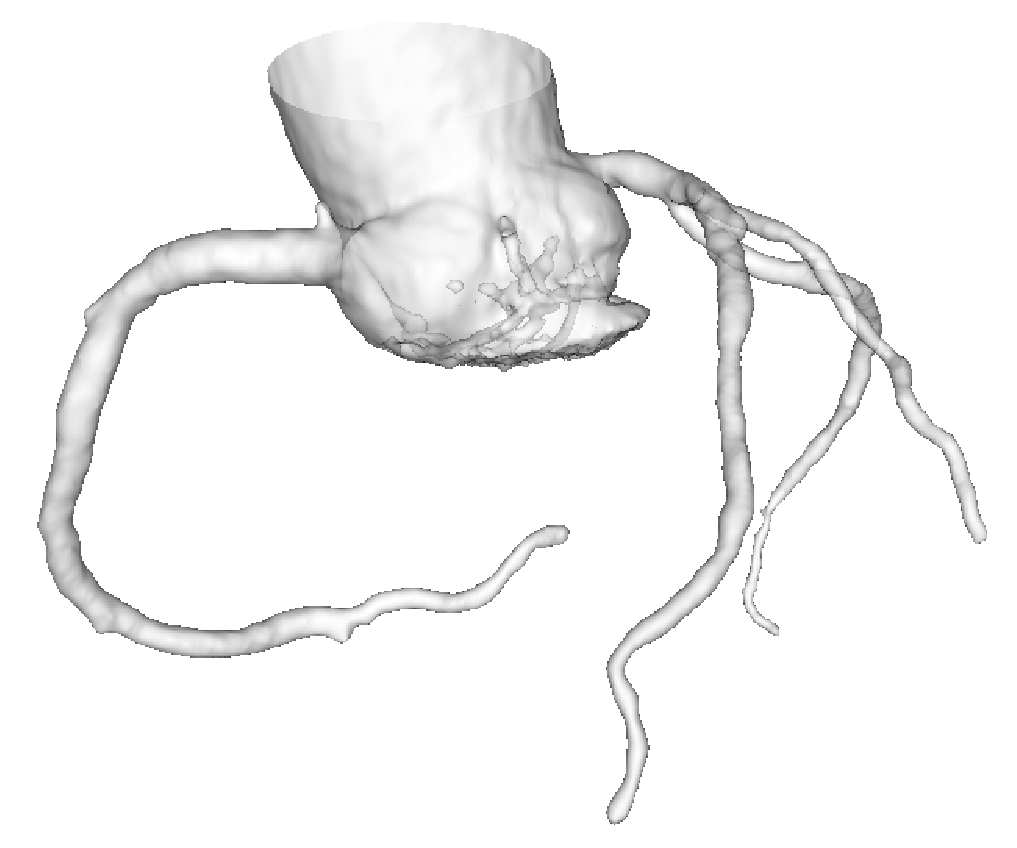
\includegraphics[height=2.5in]{Figures/coronary/model}
\caption{Surface model of coronary arteries.}%
\label{fig:coronary_CURVES_model}
\end{figure}